\chapter{Square root algorithms}

\index{square root algorithm}

A \key{square root algorithm} is an algorithm
that has a square root in its time complexity.
A square root can be seen as a ''poor man's logarithm'':
the complexity $O(\sqrt n)$ is better than $O(n)$
but worse than $O(\log n)$.
In any case, many square root algorithms are fast and usable in practice.

As an example, let us consider the problem of
creating a data structure that supports
two operations on an array:
modifying an element at a given position
and calculating the sum of elements in the given range.
We have previously solved the problem using
binary indexed and segment trees,
that support both operations in $O(\log n)$ time.
However, now we will solve the problem
in another way using a square root structure
that allows us to modify elements in $O(1)$ time
and calculate sums in $O(\sqrt n)$ time.

The idea is to divide the array into \emph{blocks}
of size $\sqrt n$ so that each block contains
the sum of elements inside the block.
For example, an array of 16 elements will be
divided into blocks of 4 elements as follows:

\begin{center}
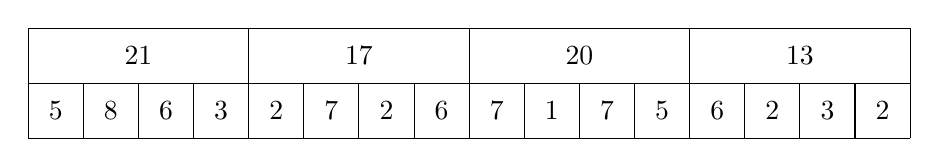
\begin{tikzpicture}[scale=0.7]
\draw (0,0) grid (16,1);

\draw (0,1) rectangle (4,2);
\draw (4,1) rectangle (8,2);
\draw (8,1) rectangle (12,2);
\draw (12,1) rectangle (16,2);

\node at (0.5, 0.5) {5};
\node at (1.5, 0.5) {8};
\node at (2.5, 0.5) {6};
\node at (3.5, 0.5) {3};
\node at (4.5, 0.5) {2};
\node at (5.5, 0.5) {7};
\node at (6.5, 0.5) {2};
\node at (7.5, 0.5) {6};
\node at (8.5, 0.5) {7};
\node at (9.5, 0.5) {1};
\node at (10.5, 0.5) {7};
\node at (11.5, 0.5) {5};
\node at (12.5, 0.5) {6};
\node at (13.5, 0.5) {2};
\node at (14.5, 0.5) {3};
\node at (15.5, 0.5) {2};

\node at (2, 1.5) {21};
\node at (6, 1.5) {17};
\node at (10, 1.5) {20};
\node at (14, 1.5) {13};

\end{tikzpicture}
\end{center}

In this structure,
it is easy to modify array elements,
because it is only needed to update
the sum of a single block
after each modification,
which can be done in $O(1)$ time.
For example, the following picture shows
how the value of an element and
the sum of the corresponding block change:

\begin{center}
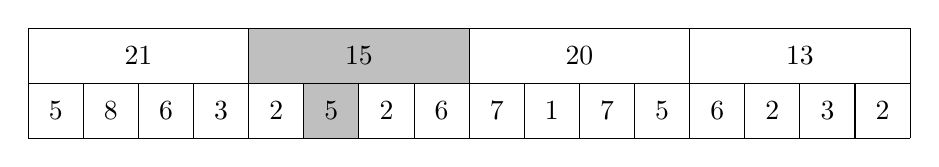
\begin{tikzpicture}[scale=0.7]
\fill[color=lightgray] (5,0) rectangle (6,1);
\draw (0,0) grid (16,1);

\fill[color=lightgray] (4,1) rectangle (8,2);
\draw (0,1) rectangle (4,2);
\draw (4,1) rectangle (8,2);
\draw (8,1) rectangle (12,2);
\draw (12,1) rectangle (16,2);

\node at (0.5, 0.5) {5};
\node at (1.5, 0.5) {8};
\node at (2.5, 0.5) {6};
\node at (3.5, 0.5) {3};
\node at (4.5, 0.5) {2};
\node at (5.5, 0.5) {5};
\node at (6.5, 0.5) {2};
\node at (7.5, 0.5) {6};
\node at (8.5, 0.5) {7};
\node at (9.5, 0.5) {1};
\node at (10.5, 0.5) {7};
\node at (11.5, 0.5) {5};
\node at (12.5, 0.5) {6};
\node at (13.5, 0.5) {2};
\node at (14.5, 0.5) {3};
\node at (15.5, 0.5) {2};

\node at (2, 1.5) {21};
\node at (6, 1.5) {15};
\node at (10, 1.5) {20};
\node at (14, 1.5) {13};

\end{tikzpicture}
\end{center}

Calculating the sum of elements in a range is
a bit more difficult.
It turns out that we can always divide
the range into three parts such that 
the sum consists of values of single elements
and sums of blocks between them:

\begin{center}
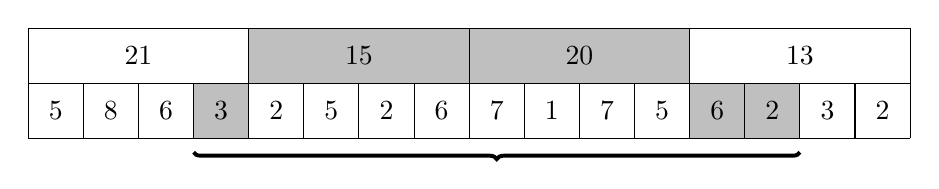
\begin{tikzpicture}[scale=0.7]
\fill[color=lightgray] (3,0) rectangle (4,1);
\fill[color=lightgray] (12,0) rectangle (13,1);
\fill[color=lightgray] (13,0) rectangle (14,1);
\draw (0,0) grid (16,1);

\fill[color=lightgray] (4,1) rectangle (8,2);
\fill[color=lightgray] (8,1) rectangle (12,2);
\draw (0,1) rectangle (4,2);
\draw (4,1) rectangle (8,2);
\draw (8,1) rectangle (12,2);
\draw (12,1) rectangle (16,2);

\node at (0.5, 0.5) {5};
\node at (1.5, 0.5) {8};
\node at (2.5, 0.5) {6};
\node at (3.5, 0.5) {3};
\node at (4.5, 0.5) {2};
\node at (5.5, 0.5) {5};
\node at (6.5, 0.5) {2};
\node at (7.5, 0.5) {6};
\node at (8.5, 0.5) {7};
\node at (9.5, 0.5) {1};
\node at (10.5, 0.5) {7};
\node at (11.5, 0.5) {5};
\node at (12.5, 0.5) {6};
\node at (13.5, 0.5) {2};
\node at (14.5, 0.5) {3};
\node at (15.5, 0.5) {2};

\node at (2, 1.5) {21};
\node at (6, 1.5) {15};
\node at (10, 1.5) {20};
\node at (14, 1.5) {13};

\draw [decoration={brace}, decorate, line width=0.5mm] (14,-0.25) -- (3,-0.25);

\end{tikzpicture}
\end{center}

Since the number of single elements is $O(\sqrt n)$
and the number of blocks is also $O(\sqrt n)$,
the time complexity of the sum query is $O(\sqrt n)$.
In this case, the parameter $\sqrt n$ balances two things:
the array is divided into $\sqrt n$ blocks,
each of which contains $\sqrt n$ elements.

In practice, it is not needed to use the
exact value of $\sqrt n$ as a parameter, but it may be better to
use parameters $k$ and $n/k$ where $k$ is
different from $\sqrt n$.
The optimal parameter depends on the problem and input.
For example, if an algorithm often goes
through the blocks but rarely inspects
single elements inside the blocks,
it may be a good idea to divide the array into
$k < \sqrt n$ blocks, each of which contains $n/k > \sqrt n$
elements.

\section{Batch processing}

\index{batch processing}

Sometimes the operations of an algorithm
can be divided into \emph{batches}.
Each batch contains a sequence of operations
which will be processed one after another.
Some precalculation is done
between the batches
in order to process the future operations more efficiently.
If there are $O(\sqrt n)$ batches of size $O(\sqrt n)$,
this results in a square root algorithm.

As an example, let us consider a problem
where a grid of size $k \times k$
initially consists of white squares
and our task is to perform $n$ operations,
each of which is one of the following:
\begin{itemize}
\item
paint square $(y,x)$ black
\item
find the nearest black square to
square $(y,x)$ where the distance
between squares $(y_1,x_1)$ and $(y_2,x_2)$
is $|y_1-y_2|+|x_1-x_2|$
\end{itemize}

We can solve the problem by dividing
the operations into
$O(\sqrt n)$ batches, each of which consists
of $O(\sqrt n)$ operations.
At the beginning of each batch,
we calculate for each square of the grid
the smallest distance to a black square.
This can be done in $O(k^2)$ time using breadth-first search.

When processing a batch, we maintain a list of squares
that have been painted black in the current batch.
The list contains $O(\sqrt n)$ elements,
because there are $O(\sqrt n)$ operations in each batch.
Now, the distance from a square to the nearest black
square is either the precalculated distance or the distance
to a square that appears in the list.

The algorithm works in
$O((k^2+n) \sqrt n)$ time.
First, there are $O(\sqrt n)$ breadth-first searches
and each search takes $O(k^2)$ time.
Second, the total number of
distances calculated during the algorithm
is $O(n)$, and when calculating each distance,
we go through a list of $O(\sqrt n)$ squares.

If the algorithm would perform a breadth-first search
at each operation, the time complexity would be
$O(k^2 n)$.
And if the algorithm would go through all painted
squares at each operation,
the time complexity would be $O(n^2)$.
Thus, the time complexity of the square root algorithm
is a combination of these time complexities,
but in addition, a factor of $n$ is replaced by $\sqrt n$.

\section{Subalgorithms}

Some square root algorithms consist of
\emph{subalgorithms} that are specialized for different
input parameters.
Typically, there are two subalgorithms:
one algorithm is efficient when
some parameter is smaller than $\sqrt n$,
and another algorithm is efficient
when the parameter is larger than $\sqrt n$.

As an example, let us consider a problem where
we are given a tree of $n$ nodes,
each with some color. Our task is to find two nodes
that have the same color and whose distance
is as large as possible.

For example, in the following tree,
the maximum distance is 4 between
the red nodes 3 and 4:

\begin{center}
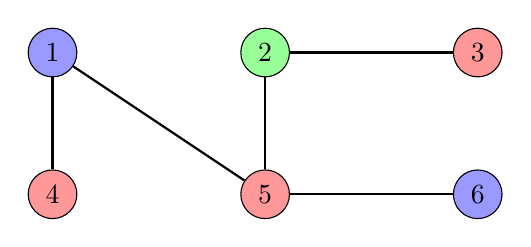
\begin{tikzpicture}[scale=0.9]
\node[draw, circle, fill=green!40] (1) at (1,3) {$2$};
\node[draw, circle, fill=red!40] (2) at (4,3) {$3$};
\node[draw, circle, fill=red!40] (3) at (1,1) {$5$};
\node[draw, circle, fill=blue!40] (4) at (4,1) {$6$};
\node[draw, circle, fill=red!40] (5) at (-2,1) {$4$};
\node[draw, circle, fill=blue!40] (6) at (-2,3) {$1$};
\path[draw,thick,-] (1) -- (2);
\path[draw,thick,-] (1) -- (3);
\path[draw,thick,-] (3) -- (4);
\path[draw,thick,-] (3) -- (6);
\path[draw,thick,-] (5) -- (6);
\end{tikzpicture}
\end{center}

The problem can be solved by going through
all colors and calculating
the maximum distance between two nodes
separately for each color.
Assume that the current color is $x$ and
there are $c$ nodes whose color is $x$.
There are two subalgorithms
that are specialized for small and large
values of $c$:

\emph{Case 1}: $c \le \sqrt n$.
If the number of nodes is small,
we go through all pairs of nodes whose
color is $x$ and select the pair that
has the maximum distance.
For each node, it is needed to calculate the distance
to $O(\sqrt n)$ other nodes (see Chapter 18.3),
so the total time needed for processing all
nodes is $O(n \sqrt n)$.

\emph{Case 2}: $c > \sqrt n$.
If the number of nodes is large,
we go through the whole tree
and calculate the maximum distance between
two nodes with color $x$.
The time complexity of the tree traversal is $O(n)$,
and this will be done at most $O(\sqrt n)$ times,
so the total time needed is $O(n \sqrt n)$.

The time complexity of the algorithm is $O(n \sqrt n)$,
because both cases take a total of $O(n \sqrt n)$ time.

\section{Integer partitions}

Some square root algorithms are based on
the following observation:
if a positive integer $n$ is represented as
a sum of positive integers,
such a sum contains only $O(\sqrt n)$ \emph{distinct} numbers.
The reason for this is that a sum with
the maximum amount of distinct numbers has to be of the form
\[1+2+3+ \cdots = n.\]
The sum of the numbers $1,2,\ldots,k$ is
\[\frac{k(k+1)}{2},\]
so the maximum amount of distinct numbers is $k = O(\sqrt n)$.
Next we will discuss two problems that can be solved
efficiently using this observation.

\subsubsection{Knapsack}

Suppose that we are given a list of integer weights
whose sum is $n$.
Our task is to find out all sums that can be formed using
a subset of the weights. For example, if the weights are
$\{1,3,3\}$, the possible sums are as follows:

\begin{itemize}[noitemsep]
\item $0$ (empty set)
\item $1$
\item $3$
\item $1+3=4$
\item $3+3=6$
\item $1+3+3=7$
\end{itemize}

Using the standard knapsack approach (see Chapter 7.4),
the problem can be solved as follows:
we define a function $f(k,s)$ whose value is 1
if the sum $s$ can be formed using the first $k$ weights,
and 0 otherwise.
All values of this function can be calculated
in $O(n^2)$ time using dynamic programming.

However, we can make the algorithm more efficient
by using the fact that the sum of the weights is $n$,
which means that there are at most $O(\sqrt n)$
distinct weights.
Thus, we can process the weights in groups
such that all weights in each group are equal.
It turns out that we can process each group
in $O(n)$ time, which yields an $O(n \sqrt n)$ time algorithm.

The idea is to use an array that records the sums of weights
that can be formed using the groups processed so far.
The array contains $n$ elements: element $k$ is 1 if the sum
$k$ can be formed and 0 otherwise.
To process a group of weights, we can easily scan the array
from left to right and record the new sums of weights that
can be formed using this group and the previous groups.

\subsubsection{String construction}

Given a string and a dictionary of words,
consider the problem of counting the number of ways
the string can be constructed using the dictionary words.
For example,
if the string is \texttt{ABAB} and the dictionary is
$\{\texttt{A},\texttt{B},\texttt{AB}\}$,
there are 4 ways:
$\texttt{A}+\texttt{B}+\texttt{A}+\texttt{B}$,
$\texttt{AB}+\texttt{A}+\texttt{B}$,
$\texttt{A}+\texttt{B}+\texttt{AB}$ and
$\texttt{AB}+\texttt{AB}$.

Assume that the length of the string is $n$
and the total length of the dictionary words is $m$.
A natural way to solve the problem is to use dynamic
programming: we can define a function $f$ such that
$f(k)$ denotes the number of ways to construct a prefix
of length $k$ of the string using the dictionary words.
Using this function, $f(n)$ gives the answer to the problem.

There are several ways to calculate the values of $f$.
One method is to store the dictionary words
in a trie and go through all ways to select the
last word in each prefix, which results in an $O(n^2)$ time algorithm.
However, instead of using a trie, we can also use string hashing
and always go through the dictionary words and compare their
hash values.

The most straightforward implementation of this idea
yields an $O(nm)$ time algorithm,
because the dictionary may contain $m$ words.
However, we can make the algorithm more efficient
by considering the dictionary words grouped by their lengths.
Each group can be processed in constant time,
because all hash values of dictionary words may be stored in a set.
Since the total length of the words is $m$,
there are at most $O(\sqrt m)$ distinct word lengths
and at most $O(\sqrt m)$ groups.
Thus, the running time of the algorithm is only $O(n \sqrt m)$.

\section{Mo's algorithm}

\index{Mo's algorithm}

\key{Mo's algorithm}\footnote{According to \cite{cod15}, this algorithm
is named after Mo Tao, a Chinese competitive programmer, but
the technique has appeared earlier in the literature \cite{ken06}.}
can be used in many problems
that require processing range queries in 
a \emph{static} array.
Since the array is static, the queries can be
processed in any order.
Before processing the queries, the algorithm
sorts them in a special order which guarantees
that the algorithm works efficiently.

At each moment in the algorithm, there is an active
range and the algorithm maintains the answer
to a query related to that range.
The algorithm processes the queries one by one,
and always moves the endpoints of the
active range by inserting and removing elements.
The time complexity of the algorithm is
$O(n \sqrt n f(n))$ when the array contains
$n$ elements, there are $n$ queries
and each insertion and removal of an element
takes $O(f(n))$ time.

The trick in Mo's algorithm is the order
in which the queries are processed:
The array is divided into blocks of $O(\sqrt n)$
elements, and the queries are sorted primarily by
the number of the block that contains the first element
in the range, and secondarily by the position of the
last element in the range.
It turns out that using this order, the algorithm
only performs $O(n \sqrt n)$ operations,
because the left endpoint moves
$n$ times $O(\sqrt n)$ steps,
and the right endpoint moves
$\sqrt n$ times $O(n)$ steps. Thus, both
endpoints move a total of $O(n \sqrt n)$ steps during the algorithm.

\subsubsection*{Example}

As an example, consider a problem
where we are given a set of queries,
each of them corresponding to a range in an array,
and our task is to calculate for each query
the number of \emph{distinct} elements in the range.

In Mo's algorithm, the queries are always sorted
in the same way, but it depends on the problem
how the answer to the query is maintained.
In this problem, we can maintain an array 
\texttt{count} where $\texttt{count}[x]$
indicates the number of times an element $x$
occurs in the active range.

When we move from one query to another query,
the active range changes.
For example, if the current range is
\begin{center}
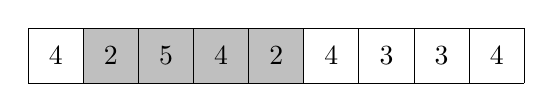
\begin{tikzpicture}[scale=0.7]
\fill[color=lightgray] (1,0) rectangle (5,1);
\draw (0,0) grid (9,1);
\node at (0.5, 0.5) {4};
\node at (1.5, 0.5) {2};
\node at (2.5, 0.5) {5};
\node at (3.5, 0.5) {4};
\node at (4.5, 0.5) {2};
\node at (5.5, 0.5) {4};
\node at (6.5, 0.5) {3};
\node at (7.5, 0.5) {3};
\node at (8.5, 0.5) {4};
\end{tikzpicture}
\end{center}
and the next range is
\begin{center}
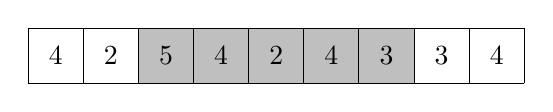
\begin{tikzpicture}[scale=0.7]
\fill[color=lightgray] (2,0) rectangle (7,1);
\draw (0,0) grid (9,1);
\node at (0.5, 0.5) {4};
\node at (1.5, 0.5) {2};
\node at (2.5, 0.5) {5};
\node at (3.5, 0.5) {4};
\node at (4.5, 0.5) {2};
\node at (5.5, 0.5) {4};
\node at (6.5, 0.5) {3};
\node at (7.5, 0.5) {3};
\node at (8.5, 0.5) {4};
\end{tikzpicture}
\end{center}
there will be three steps:
the left endpoint moves one step to the right,
and the right endpoint moves two steps to the right.

After each step, the array \texttt{count}
needs to be updated.
After adding an element $x$,
we increase the value of 
$\texttt{count}[x]$ by 1,
and if $\texttt{count}[x]=1$ after this,
we also increase the answer to the query by 1.
Similarly, after removing an element $x$,
we decrease the value of 
$\texttt{count}[x]$ by 1,
and if $\texttt{count}[x]=0$ after this,
we also decrease the answer to the query by 1.

In this problem, the time needed to perform
each step is $O(1)$, so the total time complexity
of the algorithm is $O(n \sqrt n)$.